\subsection{Aligner la caméra par rapport au faisceau laser}
\label{ssec:aligner_la_cam}
\begin{enumerate}
    \item Tourner la \textit{roulette de filtres} et sélectionner le \textit{Alexa 594} (voir figure~\ref{fig:filtres}).
        \begin{figure}[H]
        \centering
        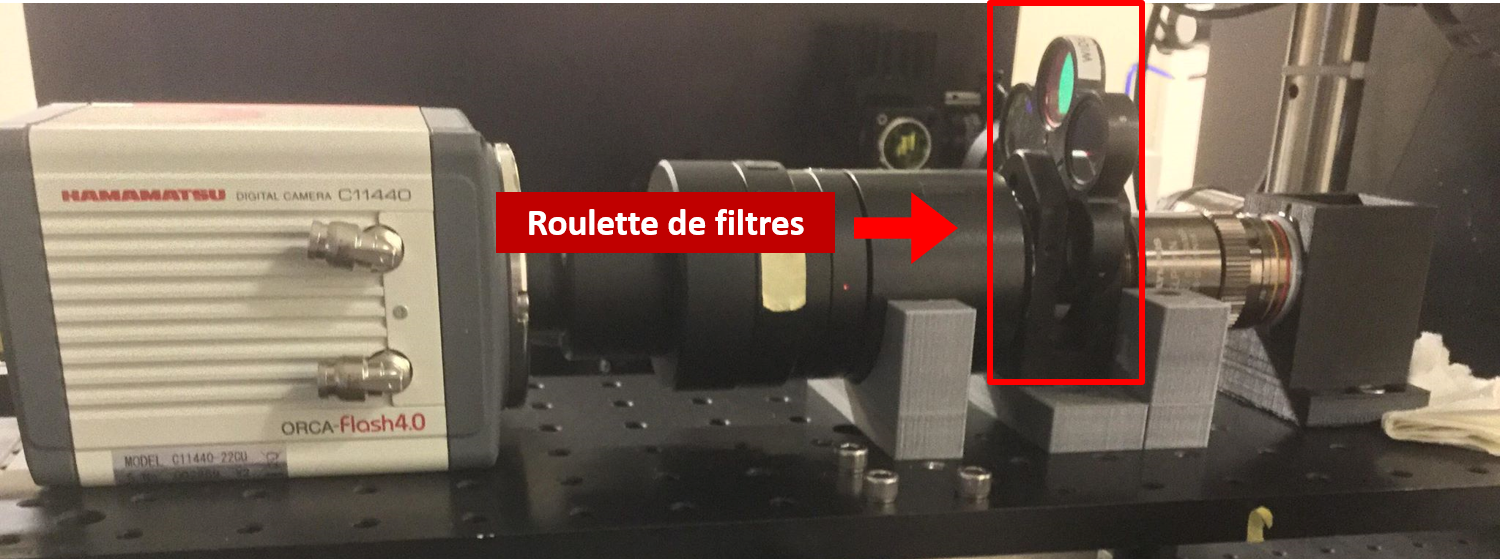
\includegraphics[width=15cm]{filtres.png}
        \caption{Roulette de filtres}
            \begin{footnotesize} \begin{description}[align=right,labelwidth=3cm]
            \item [Wide beam] Pour tout le spectre.
            \item [Alexa 488] Pour le GFP.
            \item [Alexa 568] Pour un fluorophore excité à 568~nm.
            \item [Alexa 594] Pour un fluorophore excité à 594~nm.
            \end{description} \end{footnotesize}
        \label{fig:filtres}
        \end{figure}
    \item Remplir la \textit{chambre} du liquide approprié\footnote{Le liquide de la chambre doit avoir le même indice de réfraction que l'échantillon (et que la solution dans laquelle beigne l'échantillon). Par exemple, pour un cerveau soumis à la méthode \textit{Clarity}, on peut utiliser du glycérol (n=1.47). Pour la méthode \textit{Idisco}, on peut utiliser de l'Éthyl cinnamate (n=1.52). [Attention:~Puisque l'Éthyl cinnamate a une structure moléculaire très semblable à celle du plastique, il a tendance à fuir de la chambre et à s'infiltrer dans l'objectif, ce qui finit par l'endommager grandement à long terme.]}. En mettre assez pour submerger l'objectif; ne pas trop en mettre au point où la chambre déborderait une fois la cuvette ajoutée (voir figure~\ref{fig:chambre}).
        \begin{figure}[H]
        \centering
        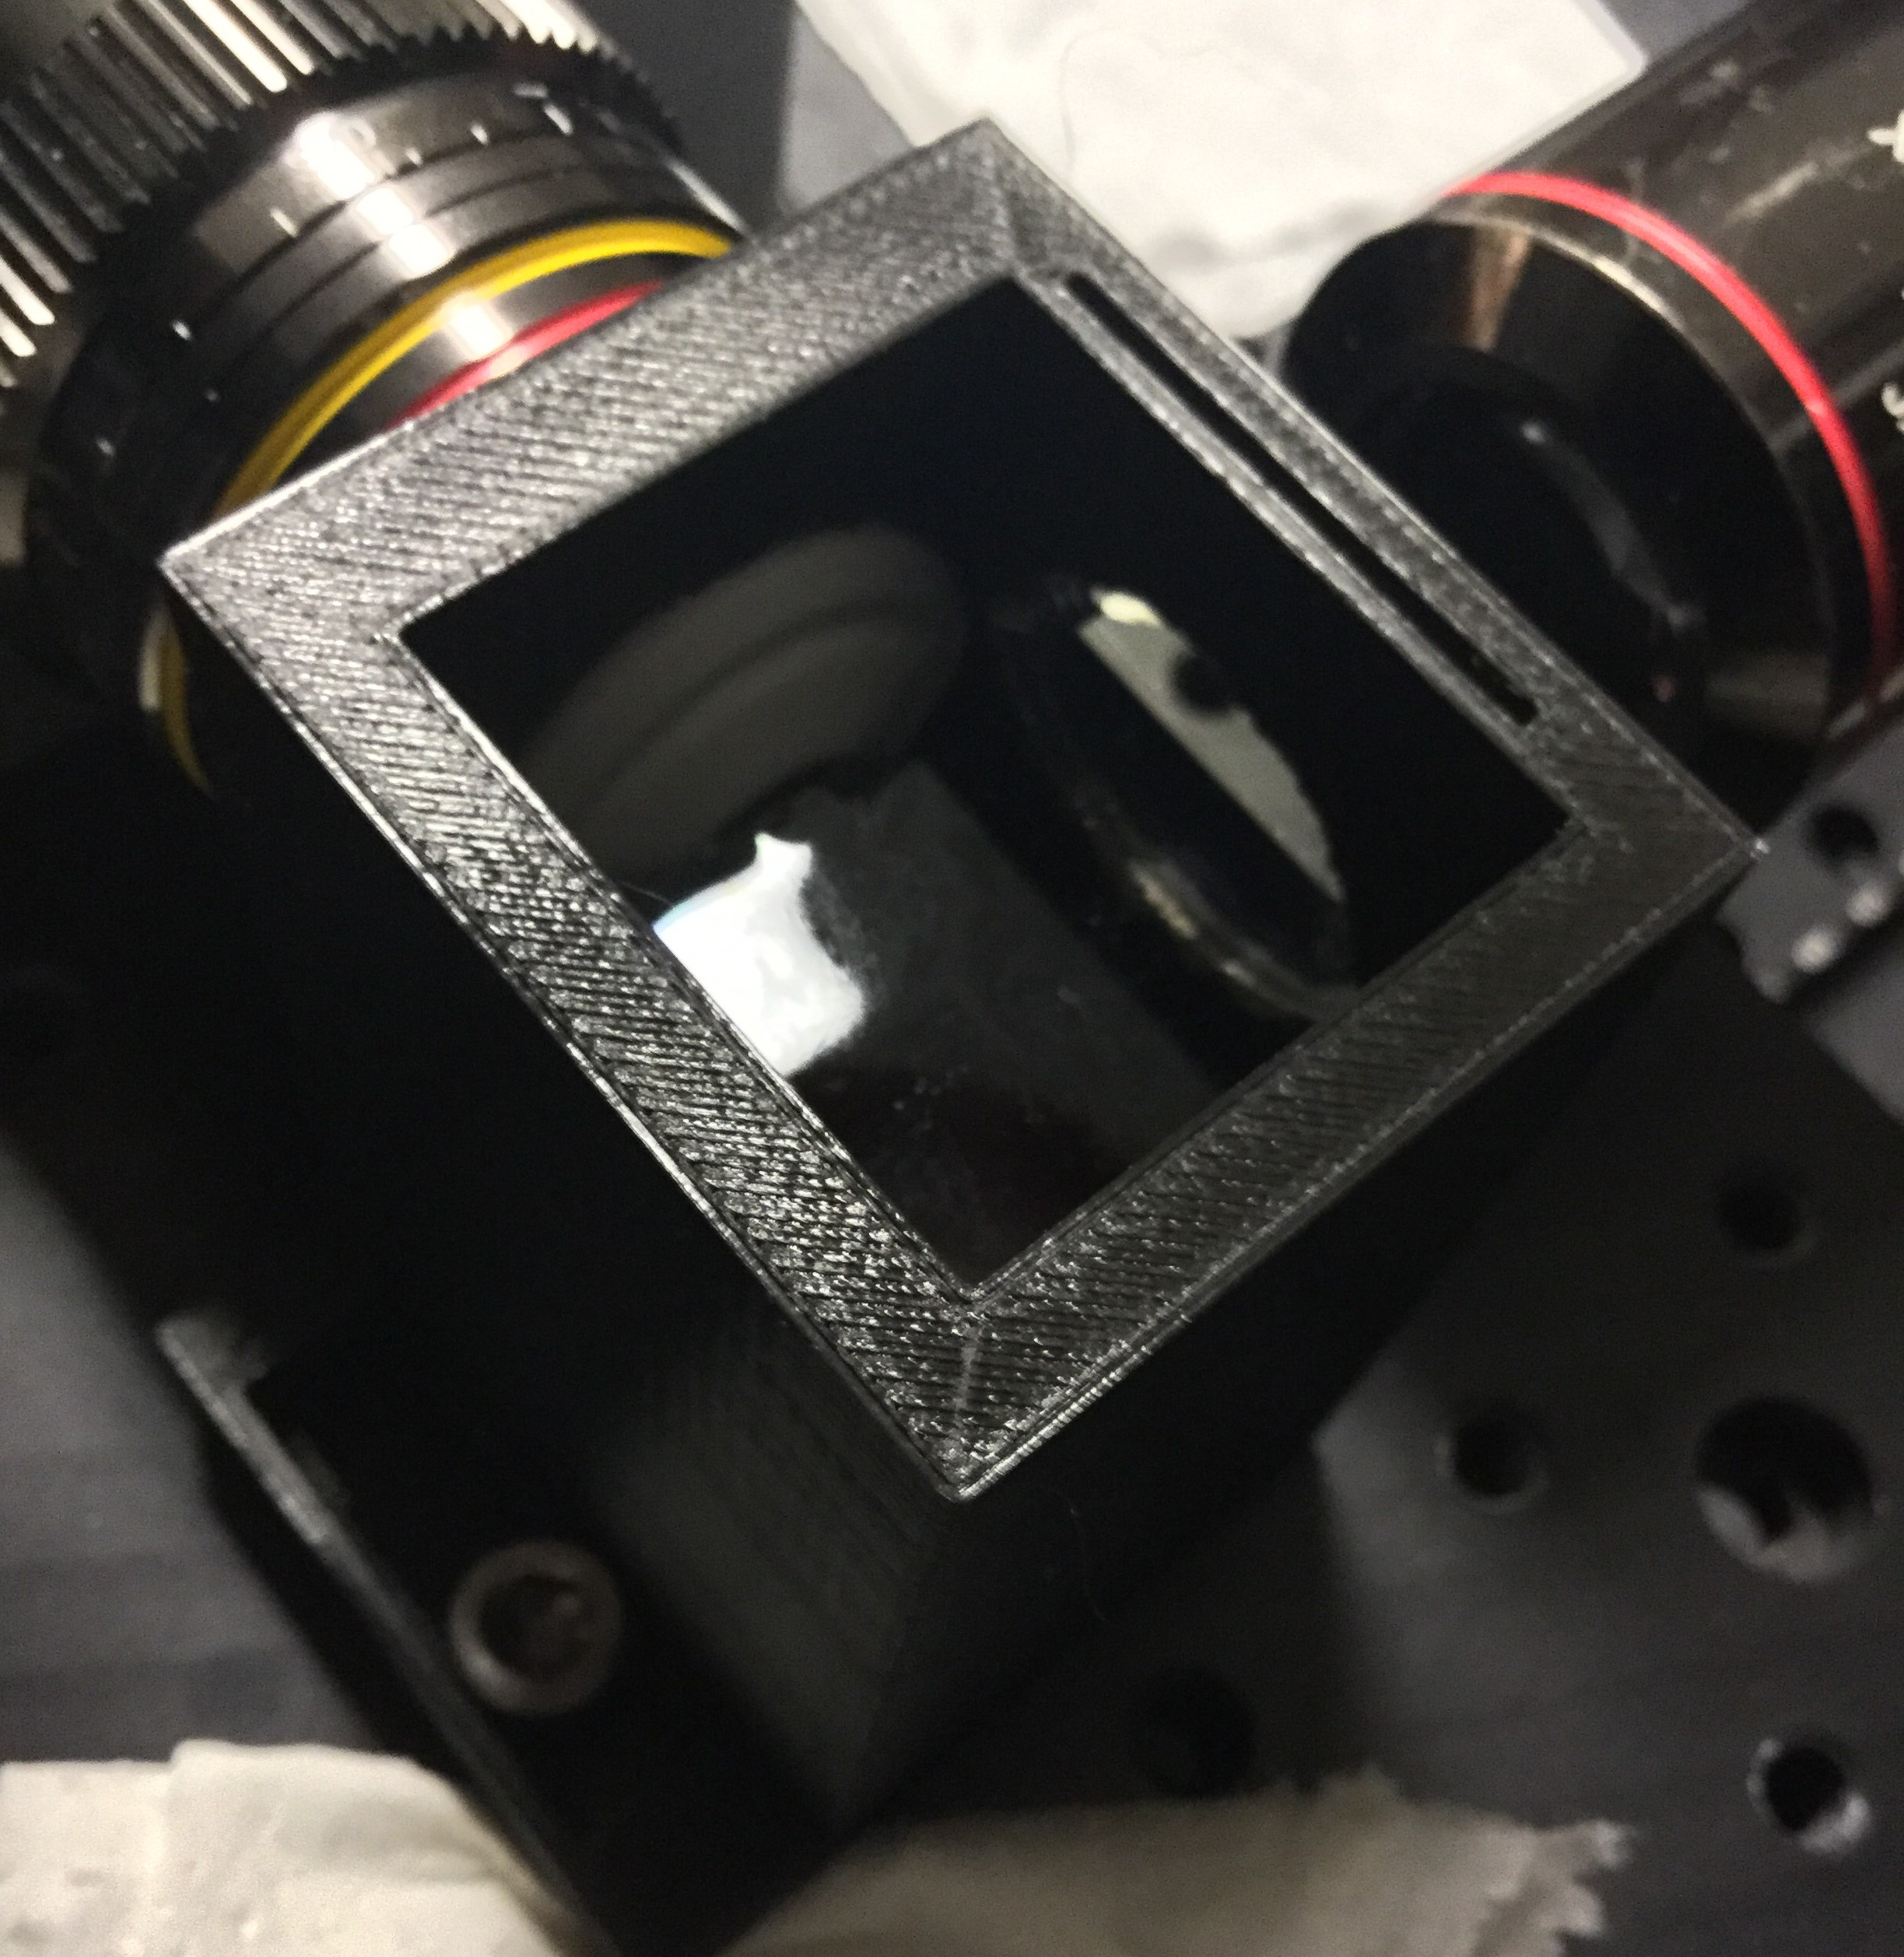
\includegraphics[width=5cm]{chambre.jpg}
        \caption{Chambre: niveau de liquide}
        \label{fig:chambre}
        \end{figure}
    \item Sortir la cuvette de \textit{solution fluorescente} (voir figure~\ref{fig:eau}).
       \begin{figure}[H]
        \centering
        \includegraphics[width=15cm]{eau.png}
        \caption{Substances à utiliser pour l'alignement de la caméra}
        \label{fig:eau}
        \end{figure}
    \item \label{ref1} Insérer cette \textit{cuvette} dans le trou au bout du \textit{support amovible} (voir figure~\ref{fig:suport}). Serrer la \textit{vis noire}.
        \begin{figure}[H]
        \centering
        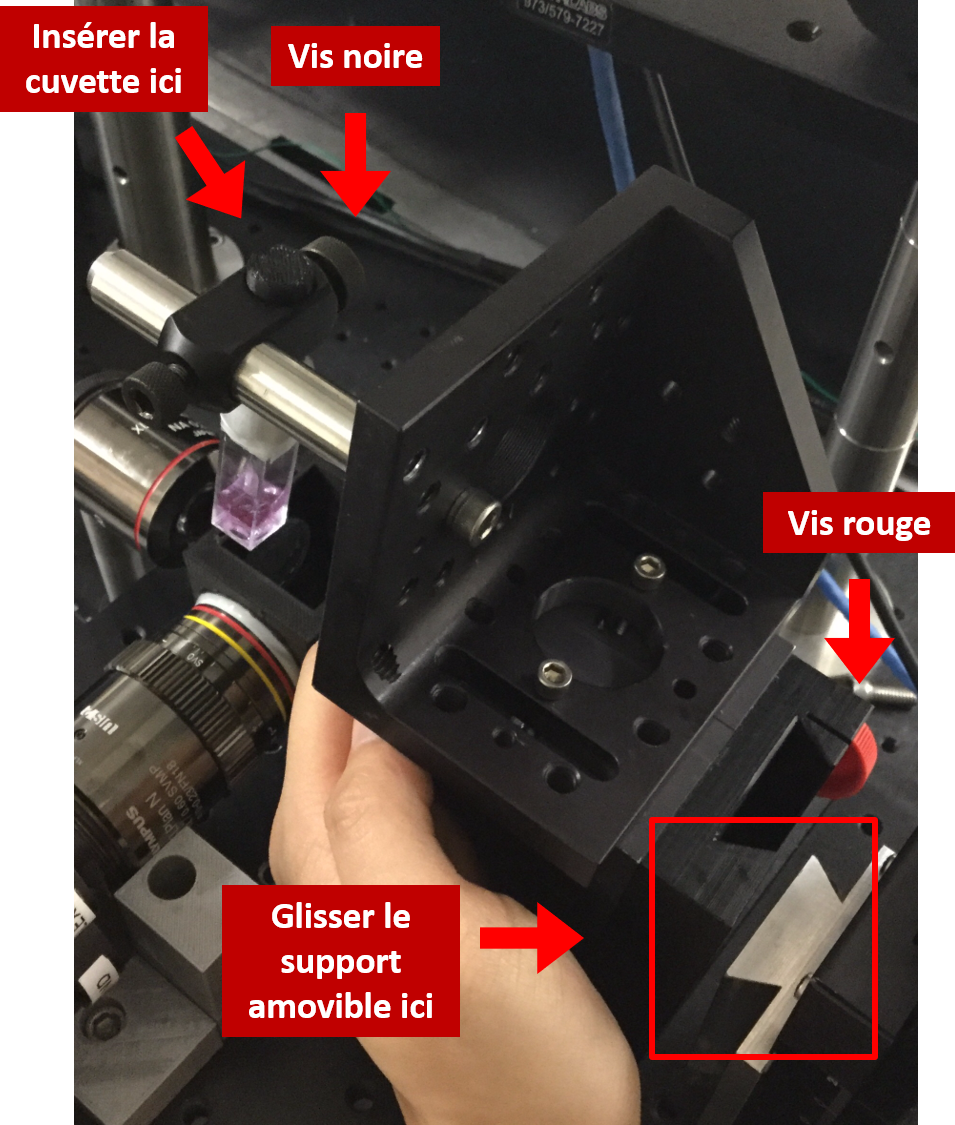
\includegraphics[width=8cm]{support.png}
        \caption{Support amovible}
        \label{fig:suport}
        \end{figure}
    \item Faire glisser le \textit{support amovible} sur la \textit{base motorisée}. Serrer la \textit{vis rouge}.
    \item  \label{ref2} A l'aide des \textit{roulettes} (voir figure~\ref{fig:roulettes}), ajuster la position de l'échantillon.
    \\ But: Voir une ligne fluorescente traverser la cuvette quand on regarde directement à l'oeil.
        \begin{figure}[H]
        \centering
        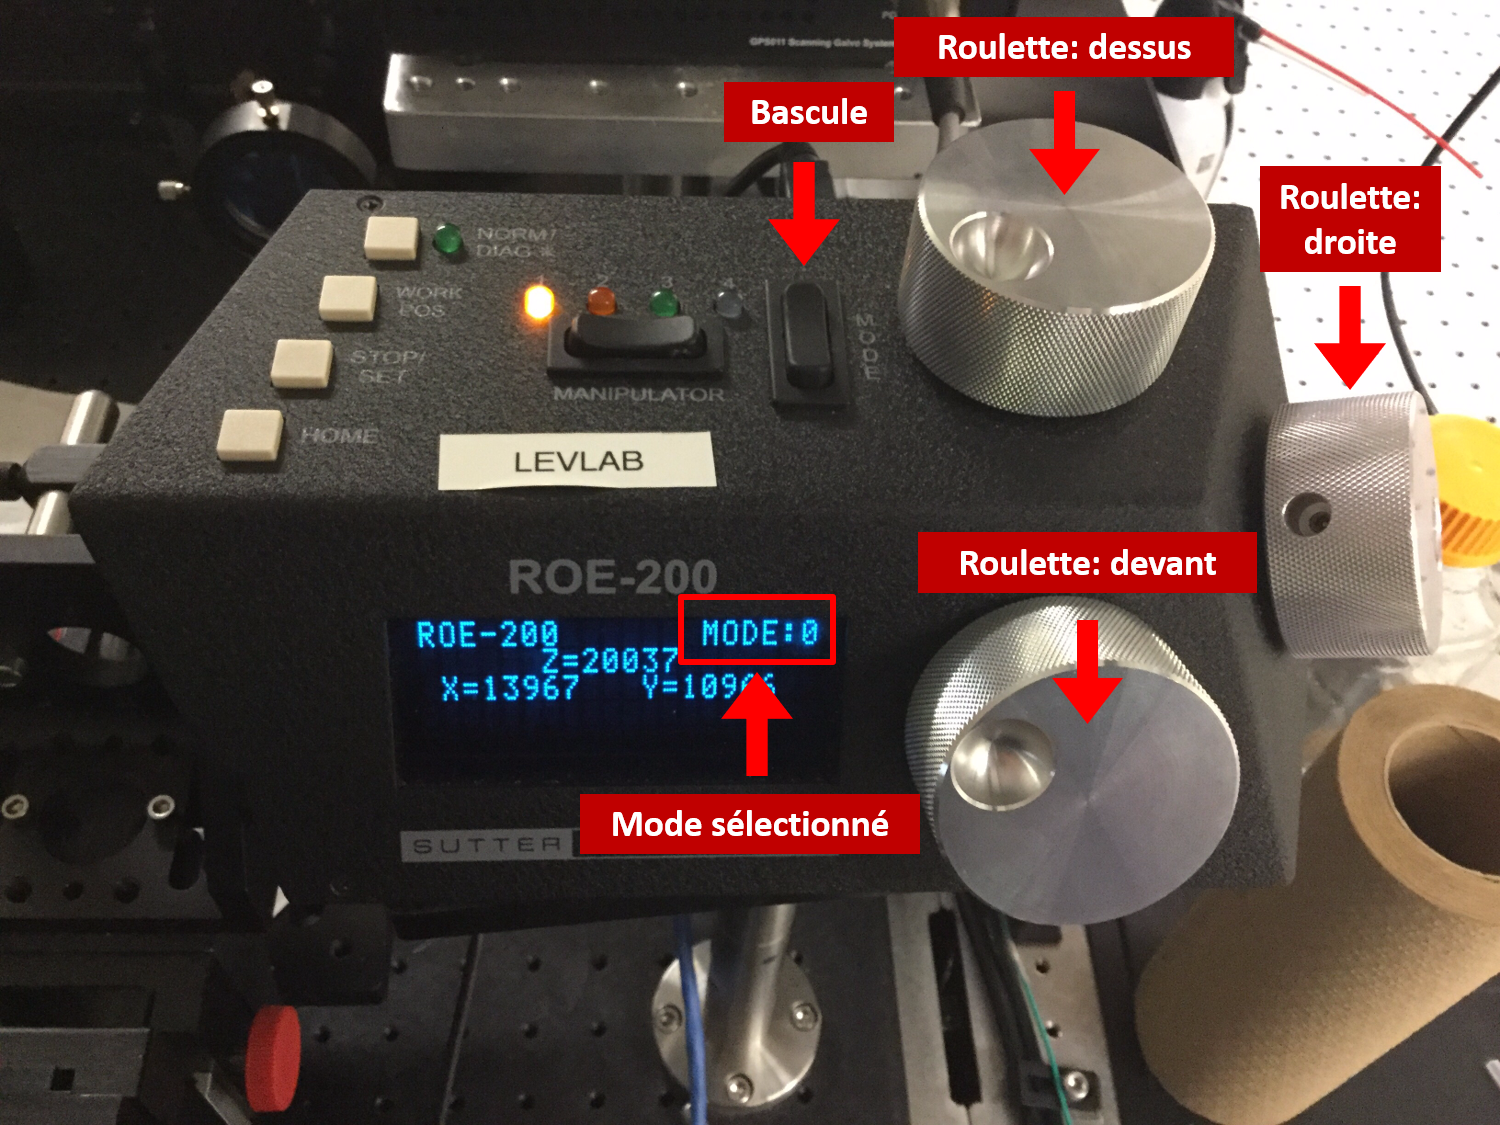
\includegraphics[width=12cm]{roulettes.png}
        \caption{Roulettes de la base motorisée}
            \begin{footnotesize} \begin{description}[align=right,labelwidth=3cm]
            \item [Roulette: dessus] Déplacement vertical. Sens horaire~=~vers le bas.
            \item [Roulette: droite] Déplacement droite-gauche. Sens horaire~=~vers la droite.
            \item [Roulette: devant] Déplacement avant-arrière. Sens horaire~=~vers l'avant.
            \item [***] \textit{Les directions sont données selon le point de vue de la photo.}
            \item [Mode] Le mode va de 0 à 9. 0~=~grands déplacements, 9~=~petits déplacements. \\ \hspace{2.2cm} On peut changer de mode en utilisant la \textit{bascule}.
            \end{description} \end{footnotesize}
        \label{fig:roulettes}
        \end{figure}
    \item Sur l'interface d'accueil (voir figure~\ref{fig:accueil}), cliquer sur \textit{Start Preview} (bouton jaune).
        \begin{figure}[H]
        \centering
        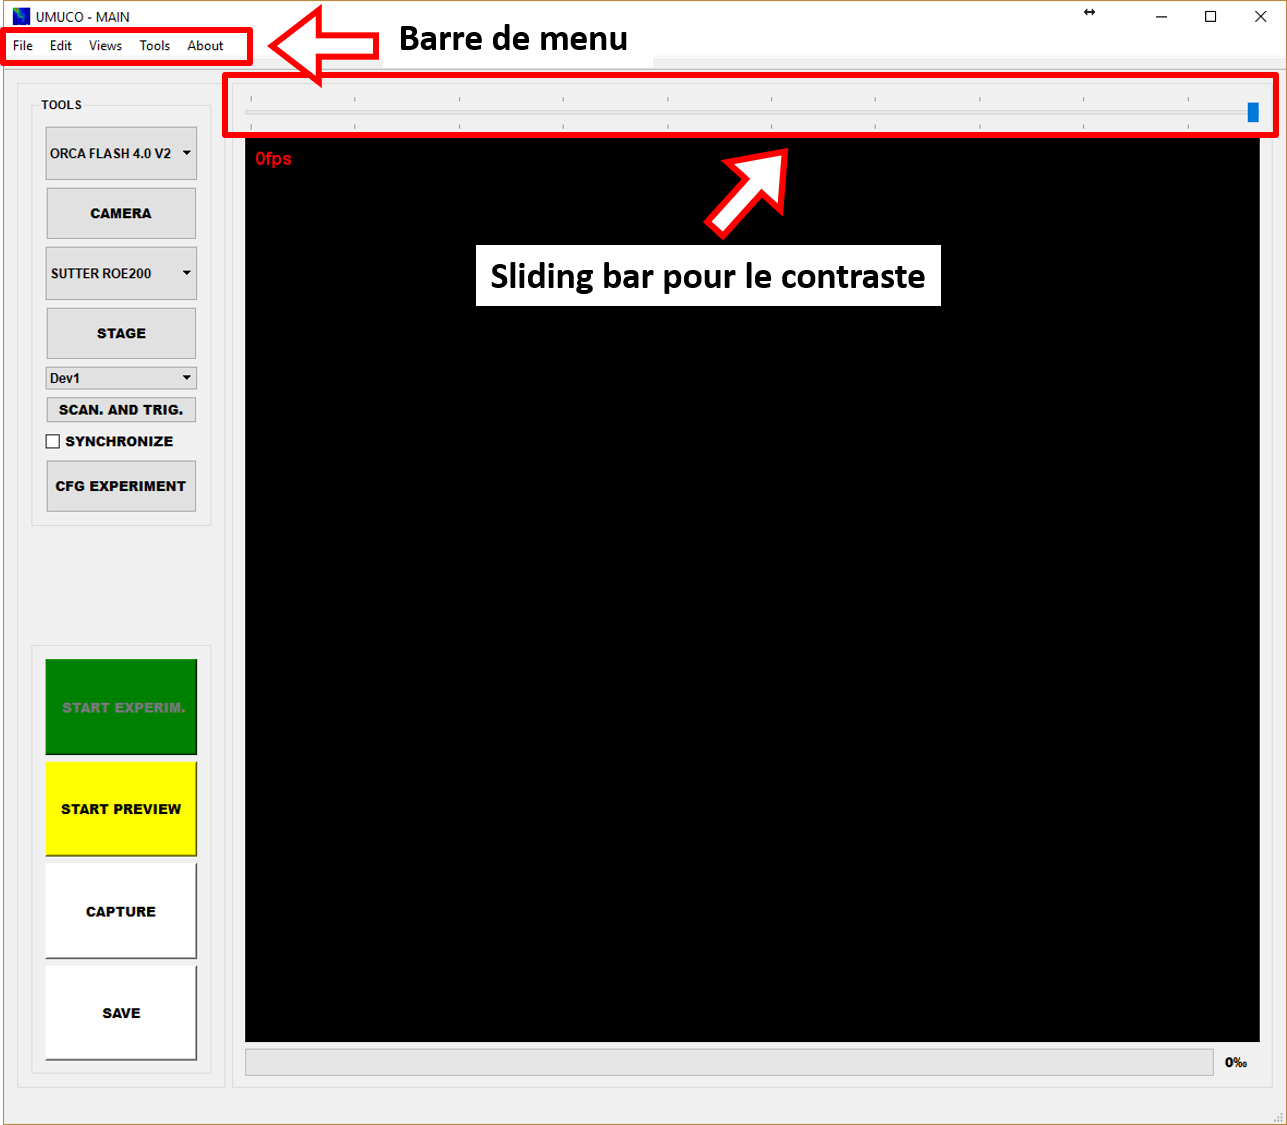
\includegraphics[width=9cm]{accueil.png}
        \caption{Interface du logiciel: accueil}
        \label{fig:accueil}
        \end{figure}
    \item Cliquer sur \textit{Scan. and Trig.} (6e bouton).
    \item Cliquer sur le menu déroulant indiqué à la figure~\ref{fig:tiret}. Sélectionner l'option '-'. Cliquer sur X pour fermer la fenêtre.
        \begin{figure}[H]
        \centering
        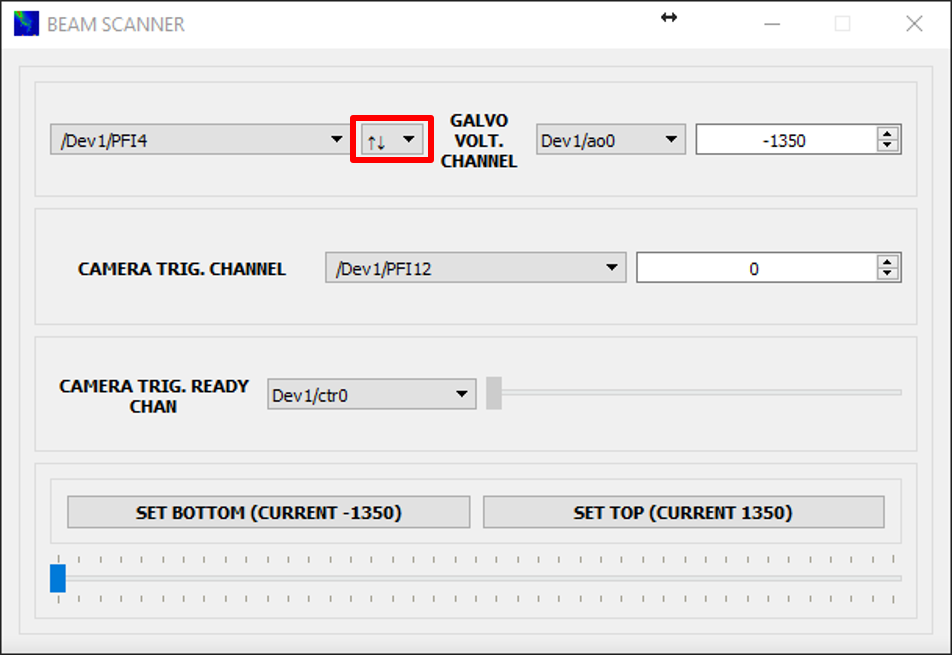
\includegraphics[width=8cm]{tiret.png}
        \caption{Fenêtre pop-up de \textit{Scan. and Trig.}}
        \label{fig:tiret}
        \end{figure}
    \item Sur l'interface d'accueil (voir figure~\ref{fig:accueil}), ajuster le contraste avec la \textit{sliding bar}. Vers la gauche~=~plus de contraste.
    \\ But: Voir du signal à l'écran, i.e. voir des picots de couleur.
        \begin{figure}[H]
        \begin{center}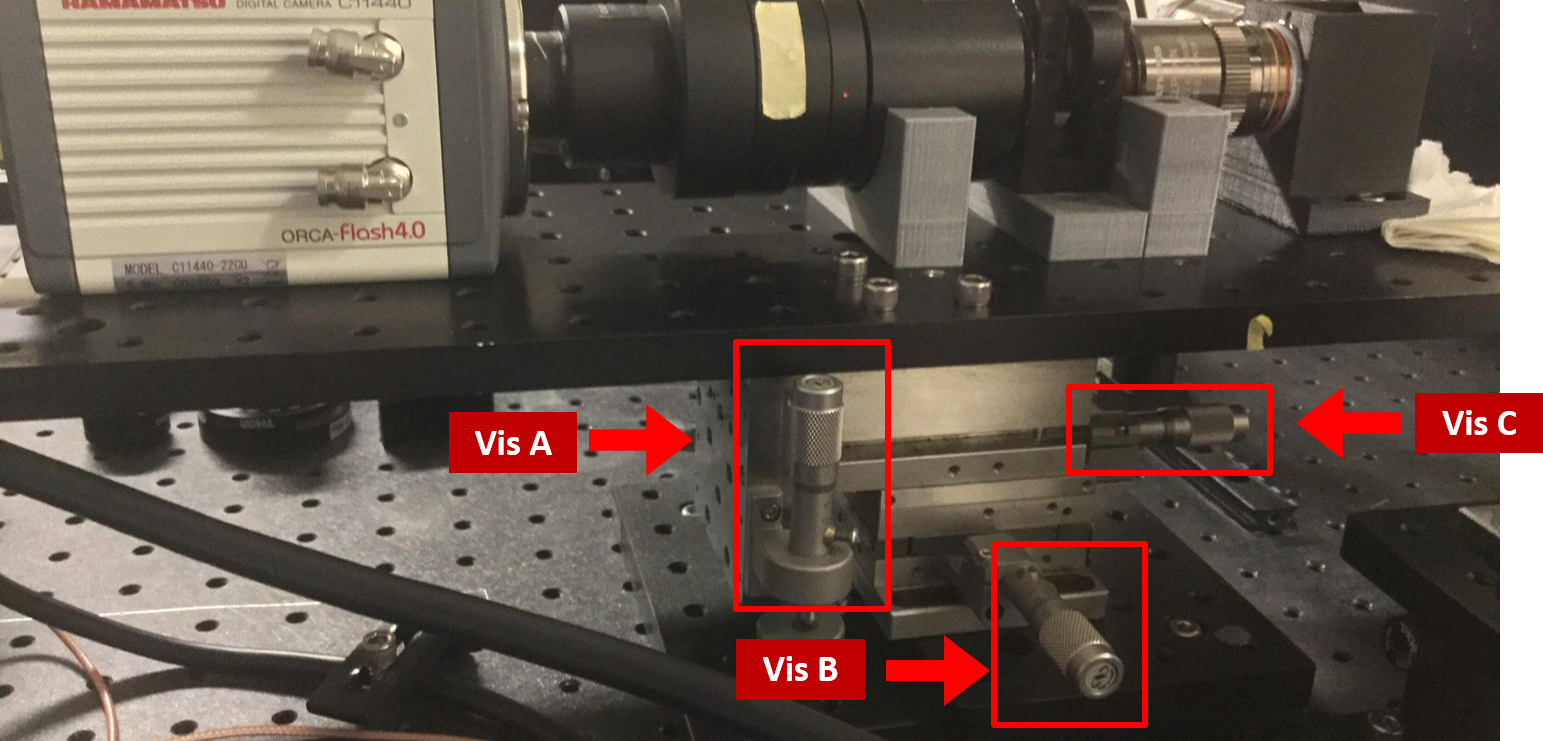
\includegraphics[width=12cm]{vis.png} \end{center}
        \caption{Vis d'ajustement du plateau de la caméra}
            \begin{footnotesize} \begin{description}[align=right,labelwidth=3cm]
            \item [Vis A] Déplacement vertical. Sens horaire~=~monter.
            \item [Vis B] Déplacement horizontal. Sens horaire~=~bouger vers la gauche.
            \item [Vis C] Déplacement en profondeur. Sens horaire~=~reculer.
            \item [***] \textit{Les directions sont données selon le point de vue de la caméra (et non de la photo).}
            \end{description} \end{footnotesize}
        \label{fig:vis}
        \end{figure}
    \item Ajuster la position verticale de la caméra à l'aide de la \textit{vis A} (voir figure~\ref{fig:vis}).
    \\ But: Voir la ligne de fluorescence. La centrer verticalement à l'écran.
    \item Ajuster la position horizontale de la caméra à l'aide de la \textit{vis B}.
    \\ But: Obtenir l'intensité la plus uniforme possible le long de la position horizontale.
    \item Ajuster la position en profondeur de la caméra à l'aide la \textit{vis C}.
    \\ But: Avoir la ligne de fluorescence au focus, i.e. avoir la ligne la plus nette/fine possible.
    \item S'aider des outils d'alignement: Dans la \textit{barre de menu} de l'interface logiciel (voir figure~\ref{fig:accueil}), cliquer sur \textit{Tools} et sur \textit{Alignment tools}.
        \begin{figure}[H]
        \centering
        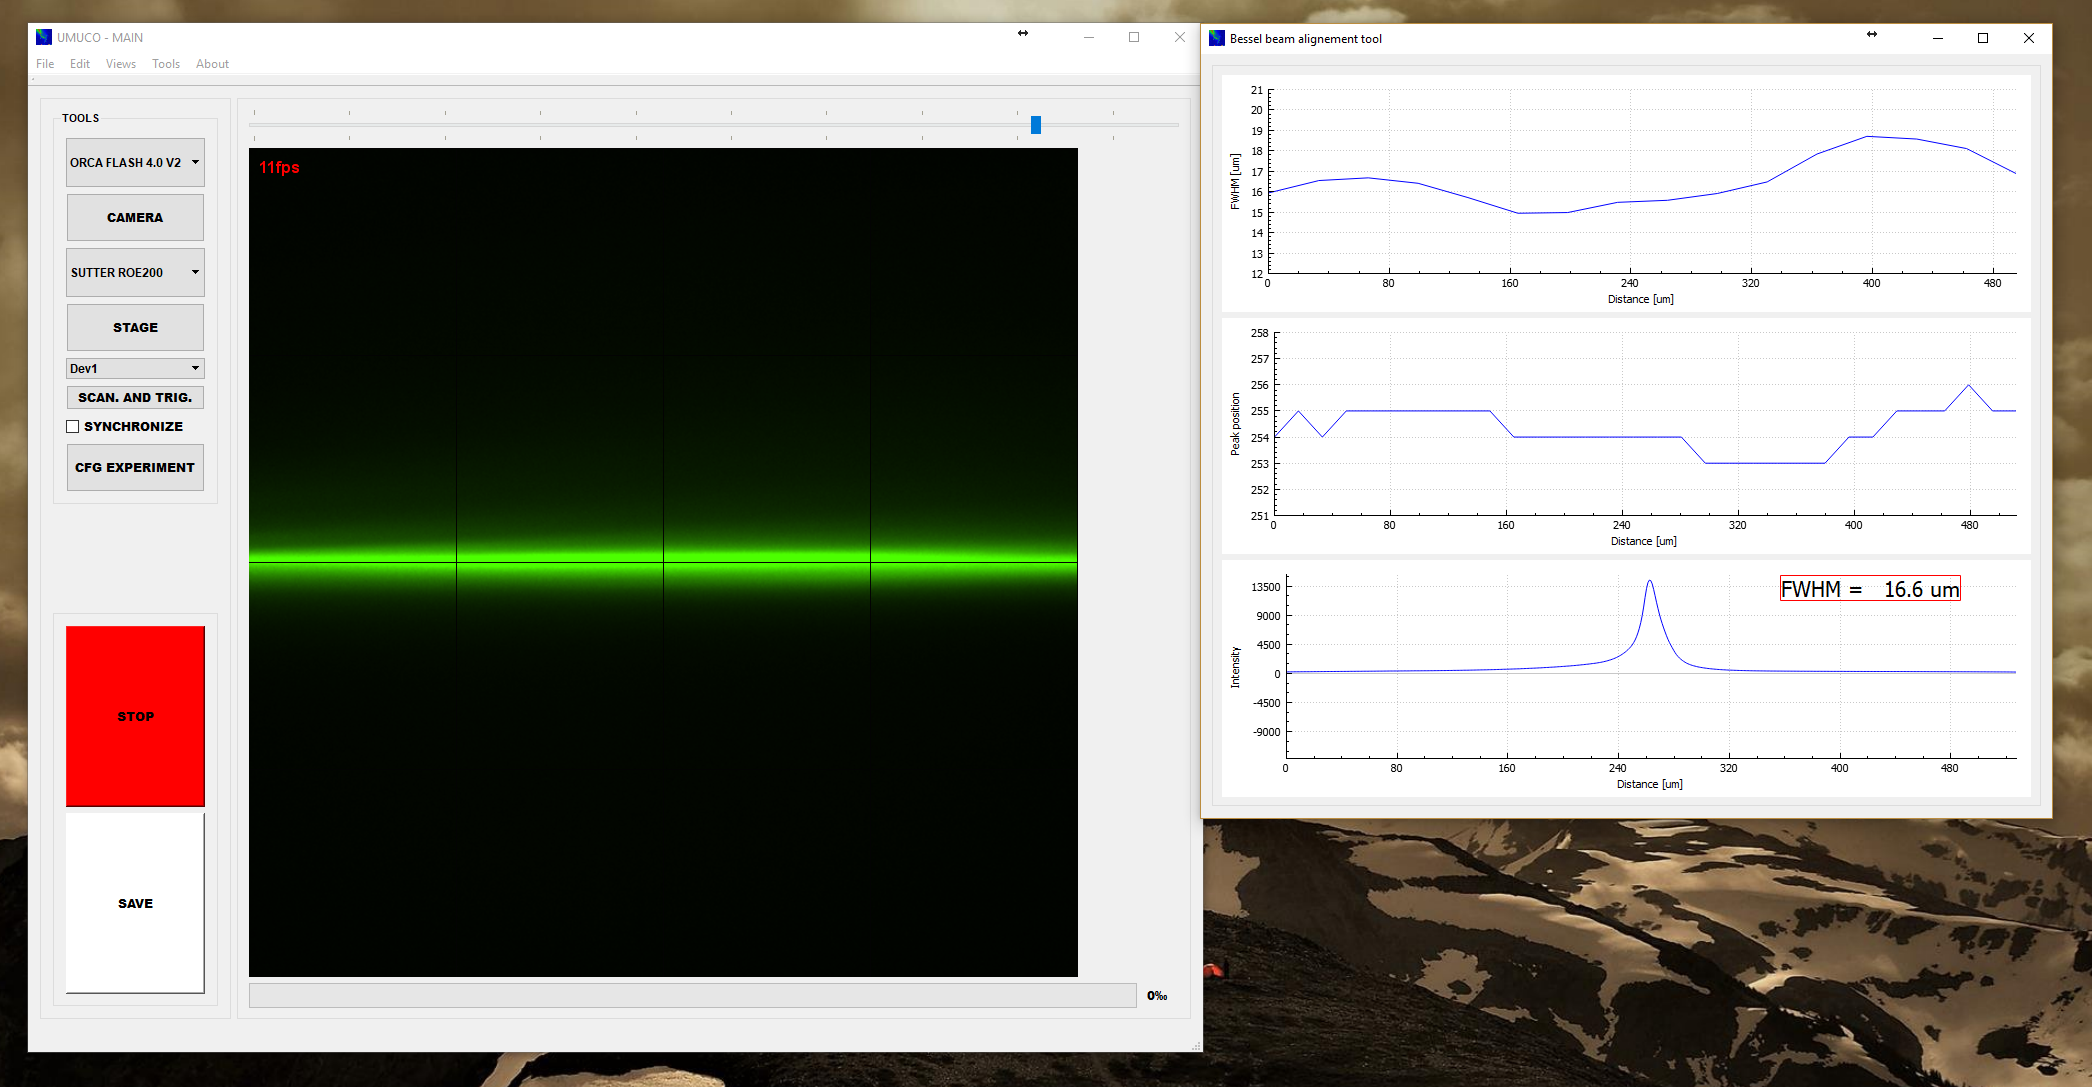
\includegraphics[width=\linewidth]{alignement.PNG}
        \caption{Outils d'alignement}
        \label{fig:alignement}
        \end{figure}
        \begin{description}[align=left,labelwidth=3cm]
        \item [FWHM against Distance] montre la largeur à mi-hauteur du profil d'intensité selon la position axiale (i.e. le long du faisceau). But: avoir une fonction constante. On peut ajuster en tournant la \textit{vis B}.
        \item [Peak Position against Distance] montre la position verticale du pic d'intensité selon la position axiale (i.e. le long du faisceau). Autrement dit, on voit si le faisceau est droit/parallèle horizontalement par rapport à la caméra. But: avoir une fonction constante. On peut ajuster en tournant la vis du bas du miroir présenté à la figure~\ref{fig:miroir}.
            \begin{figure}[H]
            \centering
            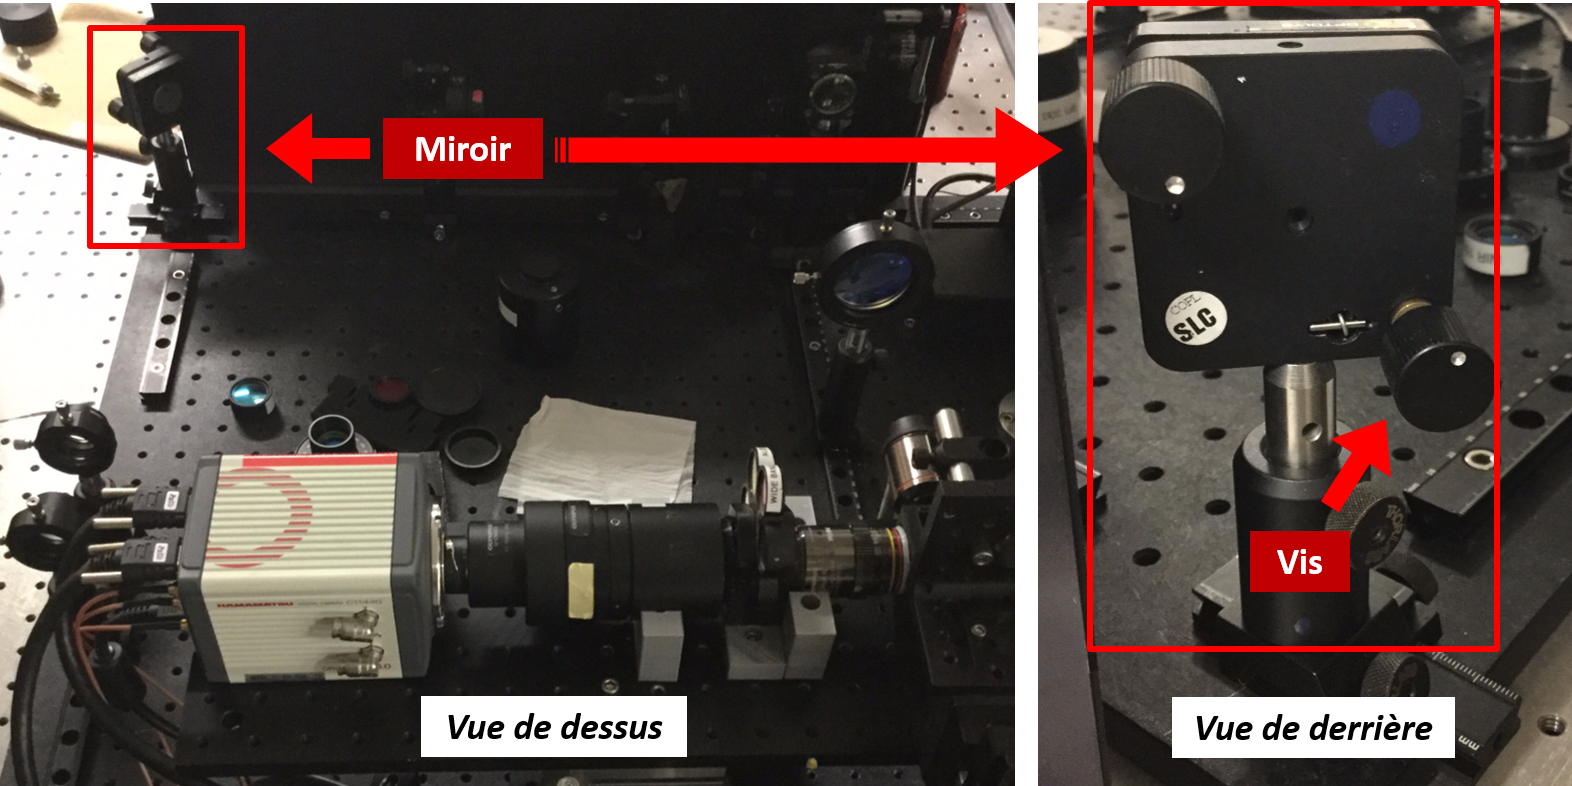
\includegraphics[width=15cm]{miroir.png}
            \caption{Miroir à ajuster}
            \label{fig:miroir}
            \end{figure}
        \item [Intensity against Distance] montre l'intensité selon la position verticale. Autrement dit, on voit le profil d'intensité du faisceau. But: avoir le pic le plus symétrique et étroit possible. La valeur du FWHM (largeur à mi-hauteur) de la courbe sur le graphique est également affichée; on veut le chiffre le plus petit. On peut ajuster en utilisant les \textit{vis B} et \textit{C}.
        \end{description}
    \item Cliquer sur X pour fermer la fenêtre d'outils d'alignement.
\end{enumerate}